\documentclass[tikz, border = 2pt]{standalone}

%---------------------------------------------------------------------------%
% PACKAGES                                                                  %
%---------------------------------------------------------------------------%

%----- MATH
%---------------------------------------------------------------------------%
\usepackage{amsmath, amssymb}

%----- FIGURES
%---------------------------------------------------------------------------%
\usepackage{pgfplots}
\pgfplotsset{compat=1.13}

\begin{document}

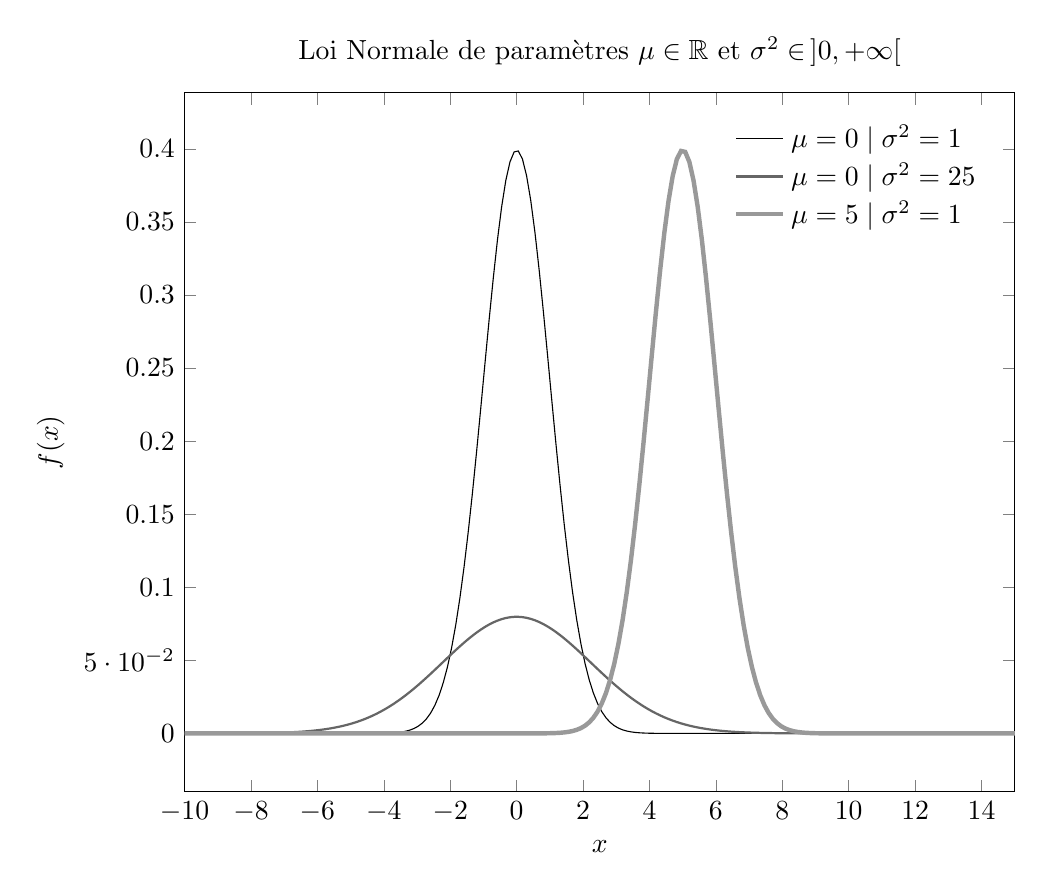
\begin{tikzpicture}
\begin{axis}[width = \textwidth,
title style = {align = center},
title={Loi Normale de param\`etres $\mu \in \mathbb{R}$ et $\sigma^2 \in\, ]0,+\infty[$},
xlabel={$x$},
ylabel={$f(x)$},
legend pos = north east,
legend style = {draw=none},
legend cell align = left,
xmin = -10,
xmax = 15,
ylabel near ticks,
domain = -10:15
]
\addplot[black, samples = 200] {(1/sqrt(2*pi))*exp(-x^2/2)};
%
\addplot[black!60, thick, samples = 200] {(1/sqrt(2*pi*25))*exp(-x^2/10)};
%
\addplot[black!40, ultra thick, samples = 200] {(1/sqrt(2*pi))*exp(-(x-5)^2/2)};
%
\legend{{$\mu=0 \mid \sigma^2 = 1$}, {$\mu=0 \mid \sigma^2 = 25$}, {$\mu=5 \mid \sigma^2 = 1$}}
\end{axis}
\end{tikzpicture}

\end{document}